\documentclass[a4paper]{article}

\usepackage[]{amsmath}
\usepackage[]{graphicx} %for includegraphics
\usepackage{epstopdf} %eps to pdf conversion with same compiler (goes after graphicx!)
\usepackage{float}

\title{Collimator simulations for development of a scanning system}

\begin{document}

\section{Collimator simulations for development of a scanning system}

A big part of the Lundium project is comprised of the development and study of a novel high purity germanium (HPGe) detector set-up.
In nuclear spectroscopy experiments in the superheavy element region the detection of x-rays is particularly interesting since they enable a pin point of the $Z$ number of the decaying nucleus. %where very exotic structures are to be studied it is necessary to employ high resolution HPGe detectors.
To increase the detection efficiency of the x-rays it is important to have a compact composition of HPGe crystals.
%In addition these detectors need to be compact to increase the detection efficiency.
The compact and x-rays together bring \textit{Compex} and this is the name of the new type of HPGe crystal detectors.
In its' beauty the HPGe set-up will consist of five so called CLOVERS, i.e. five groups of four Compex crystals brought together within a capsule.

In order to claim new nuclear structure physics it is of utmost importance to know the characteristics of the detectors, especially if it is a new type of detector.
In this regard it is hence essential to characterise the \textit{Compex} set-up in detail.

The characterisation of HPGe crystals is achieved with a scanning system.
There exist some different scanning systems \cite{phd:Dimmock, art:Crespi, art:Domingo}.
All systems utilise a collimator in some way.
The purpose of a collimator is to create a collimated $\gamma$-ray beam, a pencil beam or a focused beam with the use of an isotropical $\gamma$-ray source.

In the traditional scanning system, cf. Figure \ref{fig:livScanning}, a $\gamma$-beam is directed to one end of the crystal in a right angle.
Surrounded on the sides of the crystal other $\gamma$-detectors, such as scintillators, are placed.
With the help of slits, only $90 ^\circ$ Compton scattered $\gamma$-rays, are detected in the scintillators.
Coincidence measurements in the \textit{Compex} crystal and a scintillator determines a $\gamma$-ray interaction at a certain $(x,y,z)$ coordinate in the HPGe crystal.
With a positioning system the collimator is moved and the $(x,y)$ coordinate is varied.
With multiple slits the $z$ coordinate is varied.
This way a HPGe crystal is scanned and the response signals are studied.
%\begin{itemize}
%  \item Energy resolution
%  \item Signal amplitude
%  \item Rise time
%\end{itemize}

\begin{figure}[H]
  \centering
  \includegraphics[width=\textwidth]{/home/anton/Documents/PhD/ScanningSystem/figs_and_draws/ScanningSystem1.png}
  \caption{Liverpool scanning table \cite{phd:Dimmock}}
  \label{fig:livScanning}
\end{figure}

\begin{figure}[H]
  \centering
  \includegraphics[width=\textwidth]{/home/anton/Documents/PhD/ScanningSystem/figs_and_draws/ScanningSystem2.png}
  \caption{Measures of the Liverpool scanning table \cite{phd:Dimmock}}
  \label{fig:livScanning2}
\end{figure}

Such a scanning system is intended to be built in Lund.
A main ingredient in the scanning system is the $\gamma$-ray collimator.

%Other scanning techniques are the pulse shape comparison scan and the mix of PSCS and $\gamma$-ray imaging.
%A first intention is to characterise the \textit{Compex} crystals with the traditional technique.
%To be able to do this one needs a collimator.
Important properties of the collimator are:
\begin{itemize}
  \item Divergence of the transmitted $\gamma$-rays
  \item Scattering efficiency (full energy efficiency)
  \item Transmittance or required source activity to obtain a desired count rate in the detector
\end{itemize}
The divergence of the beam governs the position precision that is possible to obtain with the collimator. The scattering efficiency determines the amount of $\gamma$-rays that exit the collimator which have full energy. It is an important quantity since scattered particles increase the general divergence of the beam and cannot be used when the $\gamma$-ray energy is utilised in the analysis (as is the case for the system to be built in Lund). The transmittance governs the count rate in the detector and in the continuation the duration of the measurements. A known transmittance enables a well chosen source activity to obtain a desired detector count rate.

The simplest collimator is a volume with a cylinder hole where the volume can absorb $\gamma$-rays which are emitted with a too large divergence.
The scattering efficiency is not trivial to know.
A rumour said that a collimator with integrated cones actually can increase the scattering efficiency and this triggered a mini project.
In this small project, this rumour is set to test and the performance of different collimators are studied with Geant4 simulations in order to choose a suitable collimator to be used in the scanning system in Lund.

\section{Geometry definition}
The base geometry:
\begin{description}
  \item[World] $1 \times 1 \times 1$ m$^3$, air
  \item[Cylinder] Outer radius 10 cm, length 10 cm, lead. If needed an inner diameter of 1 or 1.5 mm. Placed towards the $+\hat{z}$ starting in $z = 0$.
  \item[Integrated cones] $N$ integrated cones were placed within the mother volume cylinder, with a set inner diameter to match that of the mother and an outer diameter which varied for optimised performance.
The cones were placed in such a way that the complete cylinder in $+\hat{z}$ was filled and the direction of the cones was varied with a 180$^\circ$ rotation.
The tip of the cones in the same direction of the beam was by far the best and if not otherwise mentioned (denoted flipped), it was employed.
  \item[Integrated cylinders] $N$ integrated cylinders were placed within the mother volume cylinder now with an inner diameter set to zero. Cylinders, first one with a diameter of 1 mm and then $N-1$ with a varied increasing diameter for best performance, were placed such that the cylinder with the smallest diameter was at the exit of the collimator.
\end{description}

\begin{figure}[H]
  \centering
  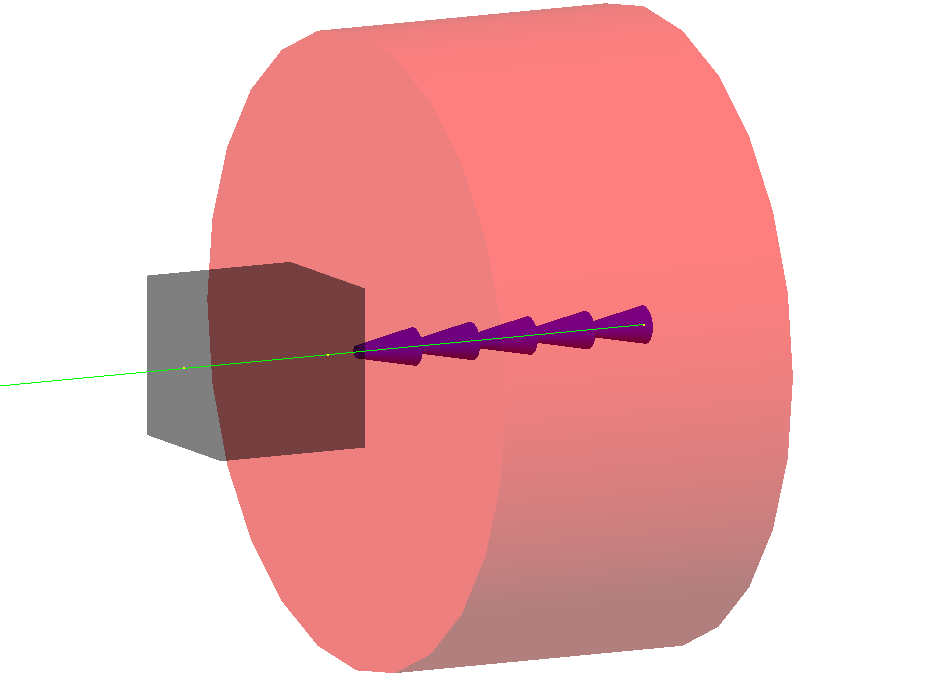
\includegraphics[width=\textwidth]{geometry.png}
  \caption{Geometry}
  \label{fig:geometry}
\end{figure}

\section{Physics model}
\begin{itemize}
  \item G4EmStandardPhysics
\end{itemize}


\section{Method}
\subsection{Primary generator}
The primary generator in Geant4 was set as follows:
\begin{description}
  \item[Type] G4ParticleGun
  \item[Particle] Gamma-photons
  \item[Position] $(0,0,0)$
  \item[Energy] $661.7$ keV to resemble a $^{137}$Cs source
  \item[Direction] $(u_x, u_y, 1)$ where:
  \begin{align}
    &u_x = r \cdot \cos \theta \\
    &u_x = r \cdot \sin \theta \\
    &\theta = \text{uniform random number}: [0, 2\pi] \\
    &r = 0.1 \cdot \sqrt{\text{uniform random number}: [0, 1]}
    \label{eq:GDir}
  \end{align}
\end{description}
\subsection{Run}
\begin{description}
  \item[Multithread] 4 parallel processes
  \item[Events] $2\cdot 10^6$
\end{description}
%A run was comprised of $2\cdot 10^6$ events. For the first run it was 100000.

\subsection{Detectors}
For the final analysis a box scoring mesh with the following settings was created:
\begin{description}
  \item[Size] $5\times5\times0.01$ cm$^3$
  \item[Location] $(0, 0, 150.0)$ mm
  \item[Binning] $500\times500$
\end{description}
I.e. it was set 5 cm from the collimator exit to resemble a real \textit{Compex} crystal scanning.

For the detailed examination with the too large inner diameter the following box scoring mesh was used:
\begin{description}
  \item[Size] $2\times2\times0.1$ cm$^3$
  \item[Location] $(0, 0, 100.5)$ mm
  \item[Binning] $200\times200$
\end{description}
I.e. it was set directly on top of the collimator exit.

A sensitive detector was set up to create an energy spectrum. It was placed 5 cm away from the collimator exit and only stored the full energy of the incoming photons.

\subsection{Analysis}
The flux (first time cm$^{-2}$) in number of $\gamma$-rays was scored with one of the built-in Geant4 scorers. Besides this, the sensitive detector scored the energy of the incoming photons and stored the energies in a histogram.
The scattering efficiency was determined as the ratio of the number of full energy $\gamma$-rays and the total detected in the sensitive detector. The beam divergence was determined as $3\sigma$ of the 2D flux. Finally, the required activity was calculated on the basis of the number of full energy $\gamma$-rays detected and the solid angle coverage:
\begin{equation}
  \Omega = \frac{\pi 15^2}{4\pi \cdot 150^2}
  \label{eq:solid_angle}
\end{equation}

\section{Results}
\begin{figure}[H]
  \centering
  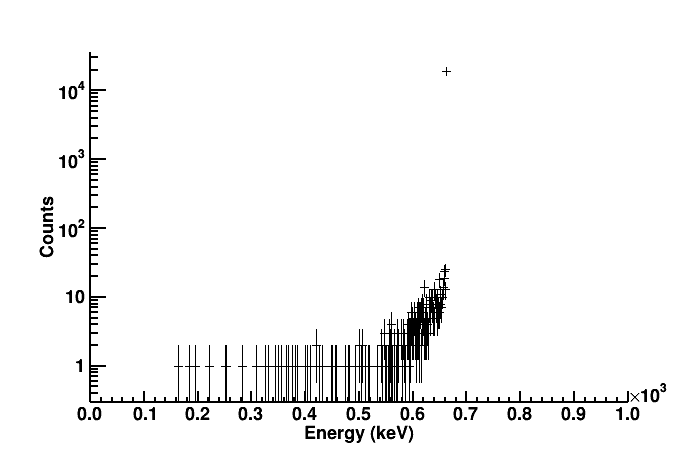
\includegraphics[width=\textwidth]{spec.png}
  \caption{Spectrum for integrated cones (i).}
  \label{fig:spec}
\end{figure}

\begin{figure}[H]
  \centering
  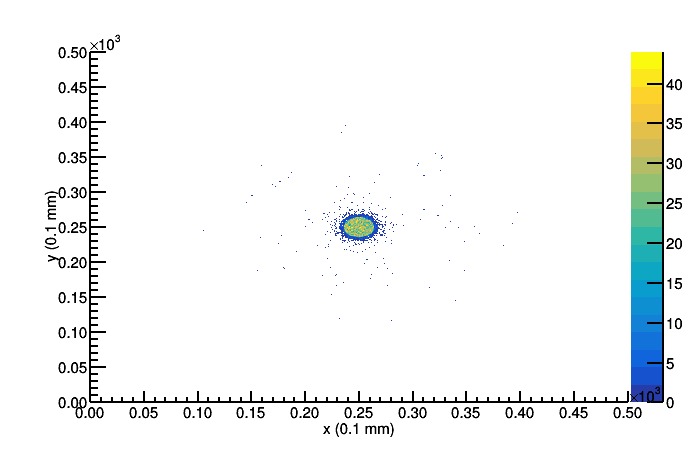
\includegraphics[width=\textwidth]{scatter.png}
  \caption{Divergence for integrated cones (i).}
  \label{fig:scatter}
\end{figure}

\begin{figure}[H]
  \centering
  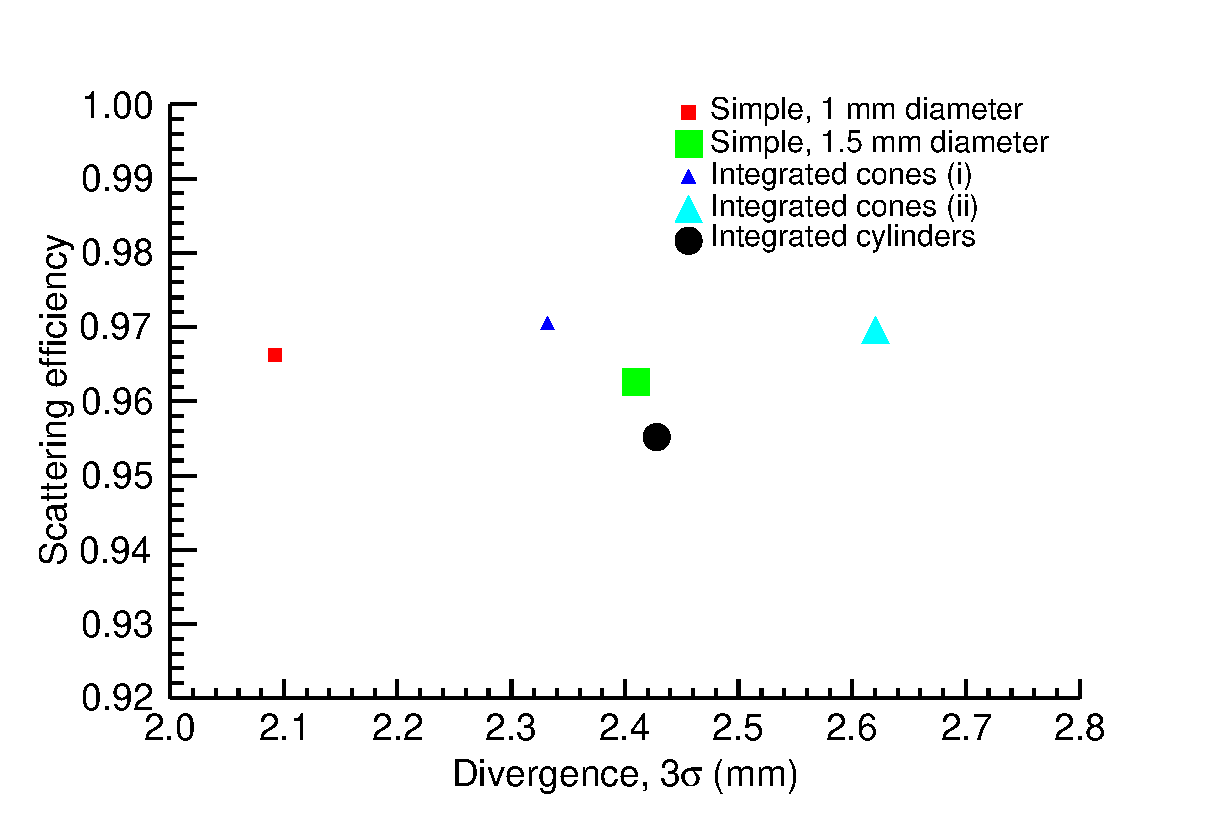
\includegraphics[width=\textwidth]{efficiency.eps}
  \caption{Results}
  \label{fig:EffvsDiv}
\end{figure}
\begin{description}
  \item[Simple, 1 mm diameter] A cylindrical collimator with diameter 1 mm.
  \item[Simple, 1.5 mm diameter] A cylindrical collimator with diameter 1.5 mm.
  \item[Integrated cones (i)] 5 cones (20 mm length) with an inner diameter of 1 mm and an outer of 1.4 mm.
  \item[Integrated cones (ii)] 5 cones (20 mm length) with an inner diameter of 1.5 mm and an outer of 1.9 mm.
  \item[Integrated cylinders] 5 cylinders (20 mm length) where the last one had a diameter of 1 mm and the rest an increasing diameter of 0.05 mm.
\end{description}

The required activity to achieve a count rate of 1 kHz for the first configuration is about 130 MBq.


\section{Conclusion}
It seems true that a collimator with integrated cones actually is able to increase the scattering efficiency, but it largely depends on the dimensions of the cones. However, many factors speak against such a configuration:
\begin{itemize}
  \item The scattering efficiency is only increased marginally.
  \item The scattering efficiency is already close to maximum with the conventional collimator type.
  \item The beam divergence increases.
  \item It is unclear of whether it is possible to manufacture such a structure.
\end{itemize}
The manufacturing possible integrated cylinder configuration did not improve on the scattering efficiency, either.
The beam divergence is rather not a measure of the spread of the beam but more a measure of leakage $\gamma$-rays making it through the lead block.

Several further configurations were investigated to see if they possibly could better optimise a collimator. These were:
\begin{itemize}
  \item Integrated cones with the end cone removed.
  \item Integrated cones separated a set distance.
  \item Integrated cones flipped.
  \item Integrated cylinders separated a set distance.
\end{itemize}
Several different dimensions were examined for the different configurations (see notes.txt in 2nd\_analysis).

\subsection{Improvements}
Possible improvements to the simulation:
\begin{itemize}
  \item Employ a biasing technique (reversed Monte Carlo, geometry based importance biasing)
\end{itemize}







\section{Shielding}
Since a very strong source is to be used,  $\sim 1$ GBq, sufficient shielding is essential to avert any radiation damages. To evaluate the amount of shielding necessary Geant4 simulations were performed.
\subsection{Geometry}
The geometry employed was very similar to the one above. The material of the cylinder was changed to wolfram and an inner diameter of 1 mm was used. An additional sensitive volume was placed with the following properties:
\begin{description}
  \item[Side box] $1\times1\times0.00001$ cm$^3$, air. Placed just on top of the cylinder collimator in $+\hat{y}$ and moved a little in $\hat{z}$ such that it was completely covered by the cylinder from the source.
\end{description}
\begin{figure}[H]
  \centering
  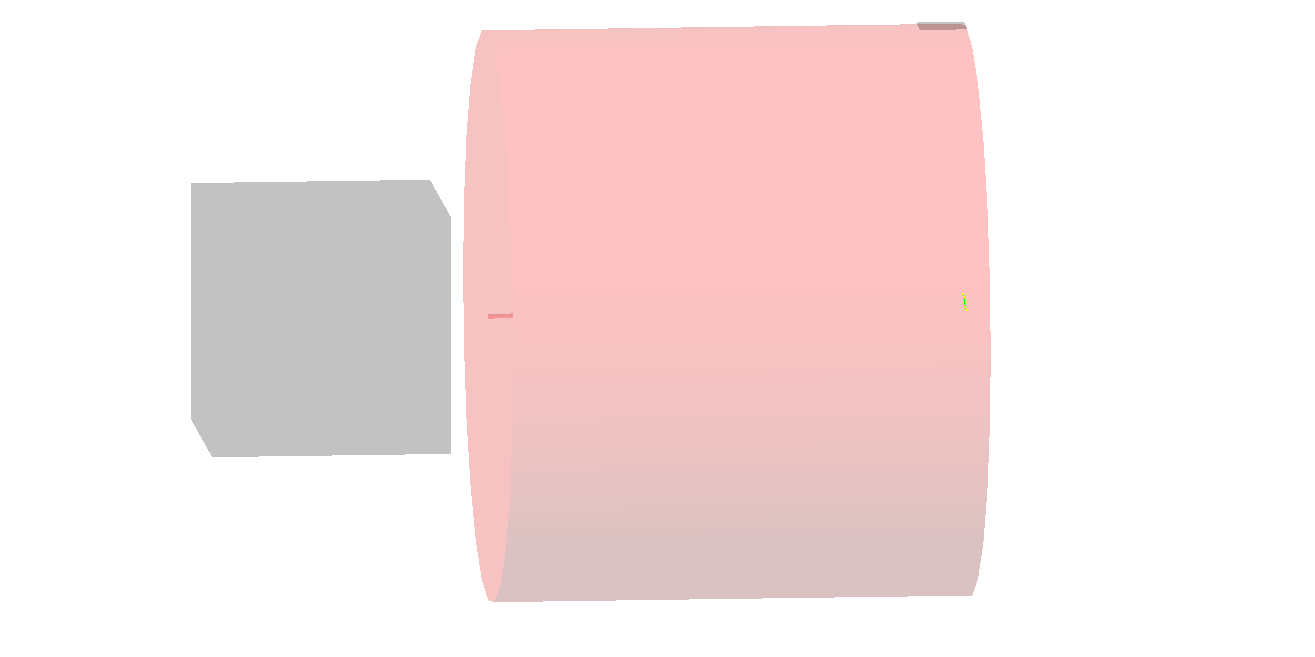
\includegraphics[width=\textwidth]{geometry2.png}
  \caption{Geometry}
  \label{fig:geometry2}
\end{figure}
\subsection{Method}
\subsubsection{Primary generator and run}
The primary generator in Geant4 was set as follows:
\begin{description}
  \item[Particle] Gamma-photons
  \item[Primary vertex] $(0,0,0)$
  \item[Energy] $661.7$ keV to resemble a $^{137}$Cs source
  \item[Direction] $(u_x, 1, u_z)$ where:
  \begin{align}
    &u_x = r \cdot \cos \theta \\
    &u_z = r \cdot \sin \theta \\
    &\theta = \text{uniform random number}: [0, \pi] \\
    &r = 0.25 \cdot \sqrt{\text{uniform random number}: [0, 1]}
    \label{eq:GDir2}
  \end{align}
\end{description}

\subsubsection{Analysis}
The box was set as a sensitive detector and the energy of the $\gamma$-rays entering the volume was stored in a histogram (just like above). In the analysis only the total histogram entries were used for the final calculations.

\subsection{Results}
The number of counts obtained with a cylinder diameter of 6 cm was 1400.
Translated into the count rate per cm$^2$ for a 1 GBq source (see 2nd\_analysis/math.py) it corresponds to:
\begin{description}
  \item[Count rate] 120 Bq/cm$^2$
  \item[Count rate around collimator] 20 kBq (based on the above number, which is exaggerated since that varies over the cylinder surface)
\end{description}

\subsection{Conclusion}
A diameter of 6 cm seems to reduce the radiation exposure around the collimator to viable levels.
For additional safety measures it will be covered with another 4 cm heavy met around the cylinder and on top and this will imply almost 100~\% shielding.




\bibliographystyle{unsrt}
\bibliography{ref}
\end{document}
